\documentclass[aspectratio=169,11pt]{beamer}

\usetheme{Madrid}
\usecolortheme{default}
\usefonttheme{professionalfonts}
\setbeamertemplate{navigation symbols}{}
\setbeamertemplate{footline}[frame number]

\usepackage{amsmath, amssymb, booktabs, graphicx}
\graphicspath{{../../assets/figures/}}

\title{What Is Behavioral Labor?}
\subtitle{Behavioral Labor --- Week 1}
\author{Teaching deck draft}
\date{}

\begin{document}

\begin{frame}
  \titlepage
\end{frame}

\begin{frame}{Central question}
\begin{itemize}
    \item What makes Behavioral Labor a coherent labor field rather than a loose application of behavioral economics?
    \item The answer starts from labor objects: work, effort, search, training, take-up, job choice, contracts, and household allocation.
    \item The course discipline: benchmark, behavioral wedge, labor margin, identification, welfare, and response.
\end{itemize}
\end{frame}

\begin{frame}{Course reorientation}
\small
\begin{tabular}{p{0.27\linewidth} p{0.63\linewidth}}
\toprule
Source course & What Behavioral Labor inherits \\
\midrule
Labor I & Worker-side labor supply, human capital, job amenities, households, and policy exposure \\
Labor II & Firms, contracts, search frictions, institutions, shocks, wage setting, and equilibrium response \\
Behavioral Labor & Preference, belief, attention, complexity, and design wedges mapped into both sides of the market \\
\bottomrule
\end{tabular}
\end{frame}

\begin{frame}{Why labor is a natural behavioral domain}
\begin{itemize}
    \item Labor decisions are repeated, high-stakes, and dynamic.
    \item Search frictions make feedback noisy and learning slow.
    \item Households and coworkers make social meaning first order.
    \item Contracts, managers, and firms shape the choice environment.
    \item Policy often works through salience, take-up, deadlines, and complexity.
\end{itemize}
\end{frame}

\begin{frame}{Benchmark labor model}
\[
a_i^\star \in \arg\max_{a \in \mathcal{A}} U_i(a;\theta_i)
\quad \text{s.t.} \quad c_i = g(a,p,y_i)
\]

\begin{itemize}
    \item $a$ may be hours, effort, search intensity, training, applications, job choice, or take-up.
    \item The benchmark is a serious starting point, not a straw model.
    \item Behavioral Labor asks whether the worker solves the same problem the analyst writes down.
\end{itemize}
\end{frame}

\begin{frame}{Behavioral wedge representation}
\[
a_i^{B} \in \arg\max_{a \in \mathcal{A}_i(\lambda_i)}
\tilde{U}_i(a;\theta_i,\beta_i,r_i,\eta_i)
\quad \text{s.t.} \quad \tilde{g}_i(a \mid b_i,\lambda_i)
\]

\small
\begin{tabular}{p{0.20\linewidth} p{0.68\linewidth}}
\toprule
Object & Interpretation \\
\midrule
$\beta_i,r_i,\eta_i$ & present bias, reference points, reciprocity, social preferences, identity \\
$b_i$ & subjective beliefs and expectations \\
$\lambda_i$ & attention, salience, complexity, limited consideration \\
$\tilde{g}_i$ & perceived or designed environment, including firm and policy response \\
\bottomrule
\end{tabular}
\end{frame}

\begin{frame}{DellaVigna taxonomy adapted to labor}
\begin{center}
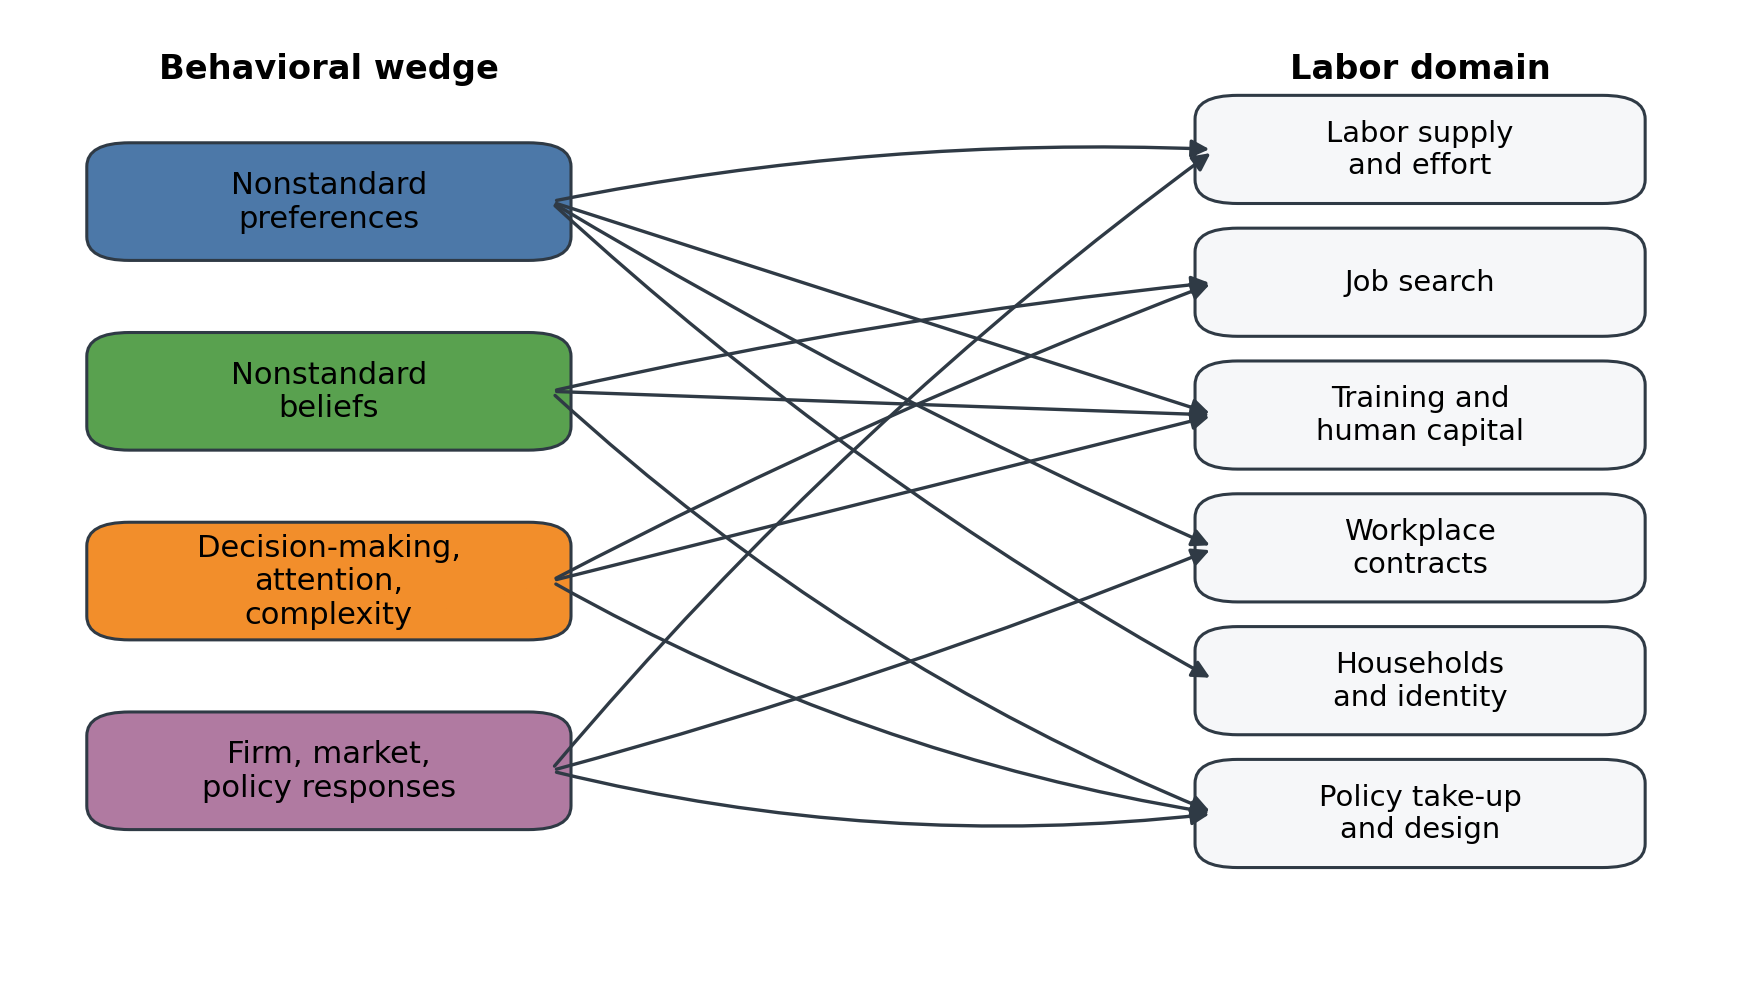
\includegraphics[height=0.78\textheight,keepaspectratio]{01-taxonomy-to-labor-domains.png}
\end{center}
\end{frame}

\begin{frame}{Labor domains where behavioral frictions matter}
\small
\begin{tabular}{p{0.30\linewidth} p{0.56\linewidth}}
\toprule
Domain & Behavioral question \\
\midrule
Labor supply and effort & Do incentives create durable effort or only short-run response? \\
Job search & Do beliefs and motivation change search intensity and job finding? \\
Training and human capital & Why is investment low when returns may be delayed and uncertain? \\
Workplace contracts & Do fairness, reciprocity, or complexity change productivity? \\
Households and identity & Do norms alter labor supply and specialization? \\
Policy take-up & Do workers notice, understand, and act on the program? \\
\bottomrule
\end{tabular}
\end{frame}

\begin{frame}{Benchmark versus behavioral wedges}
\begin{center}
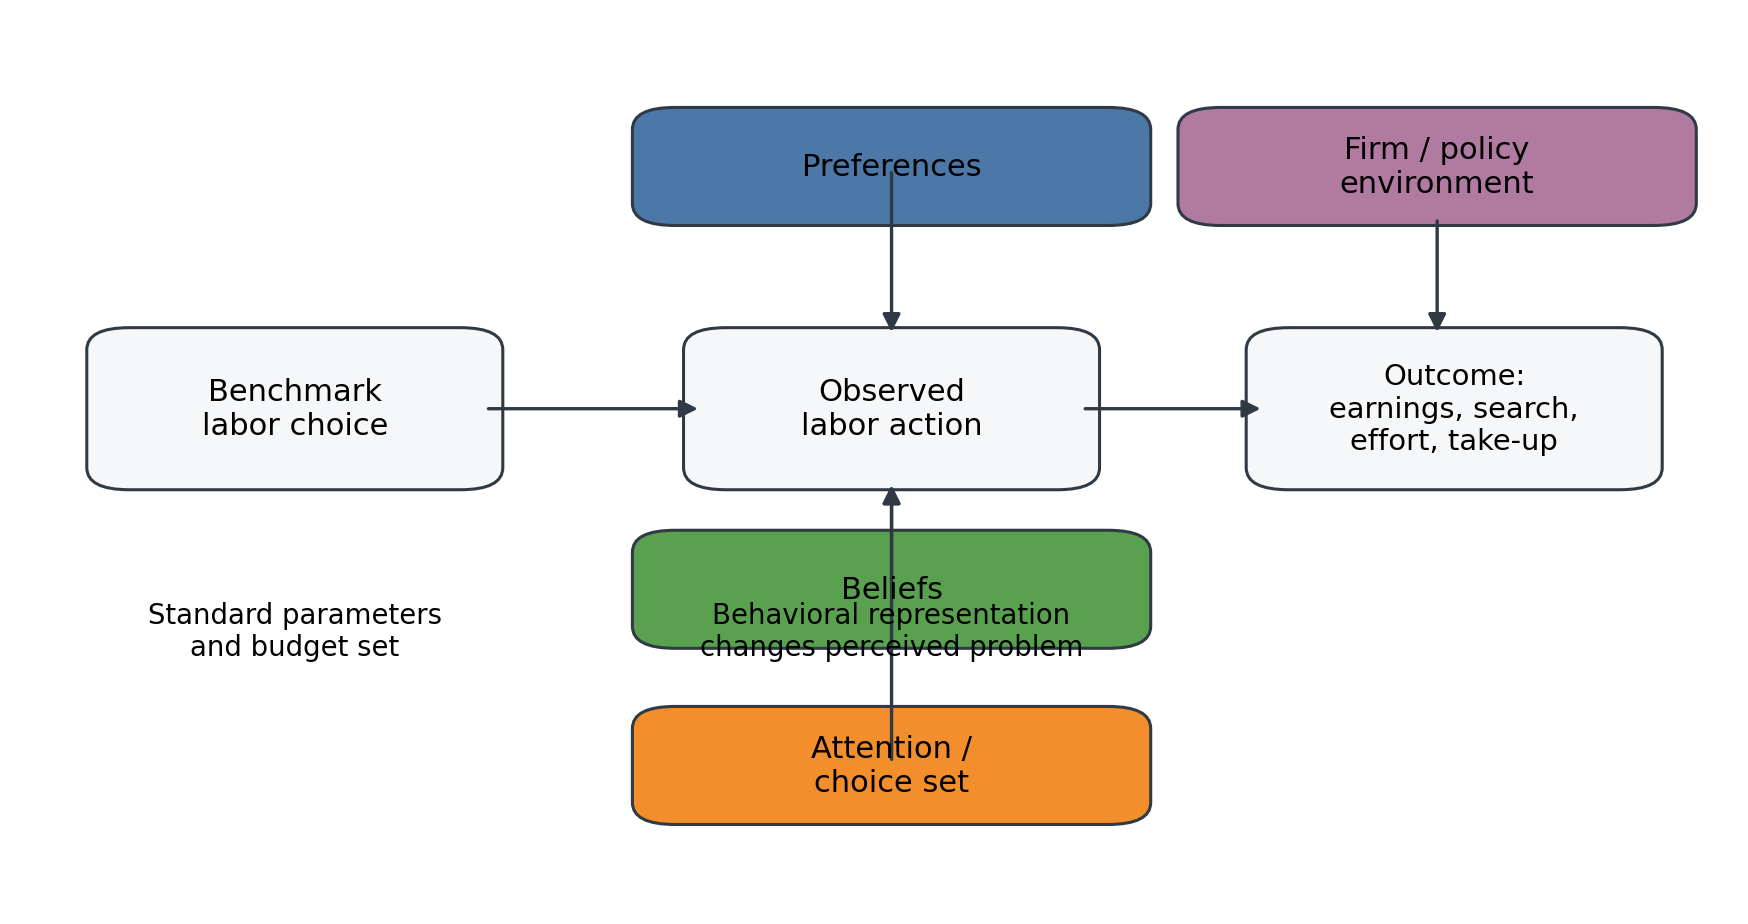
\includegraphics[height=0.76\textheight,keepaspectratio]{01-benchmark-vs-behavioral-wedge.png}
\end{center}
\end{frame}

\begin{frame}{Examples: workers, households, firms, policy}
\begin{itemize}
    \item Workers: commitment demand, habit formation, search motivation, perceived returns.
    \item Households: identity costs and relative income can shape labor allocation.
    \item Firms: managers can simplify, frame, monitor, screen, or offer commitment.
    \item Policy: statutory generosity differs from effective exposure when take-up is costly or confusing.
\end{itemize}
\end{frame}

\begin{frame}{Methods and identification}
\begin{center}
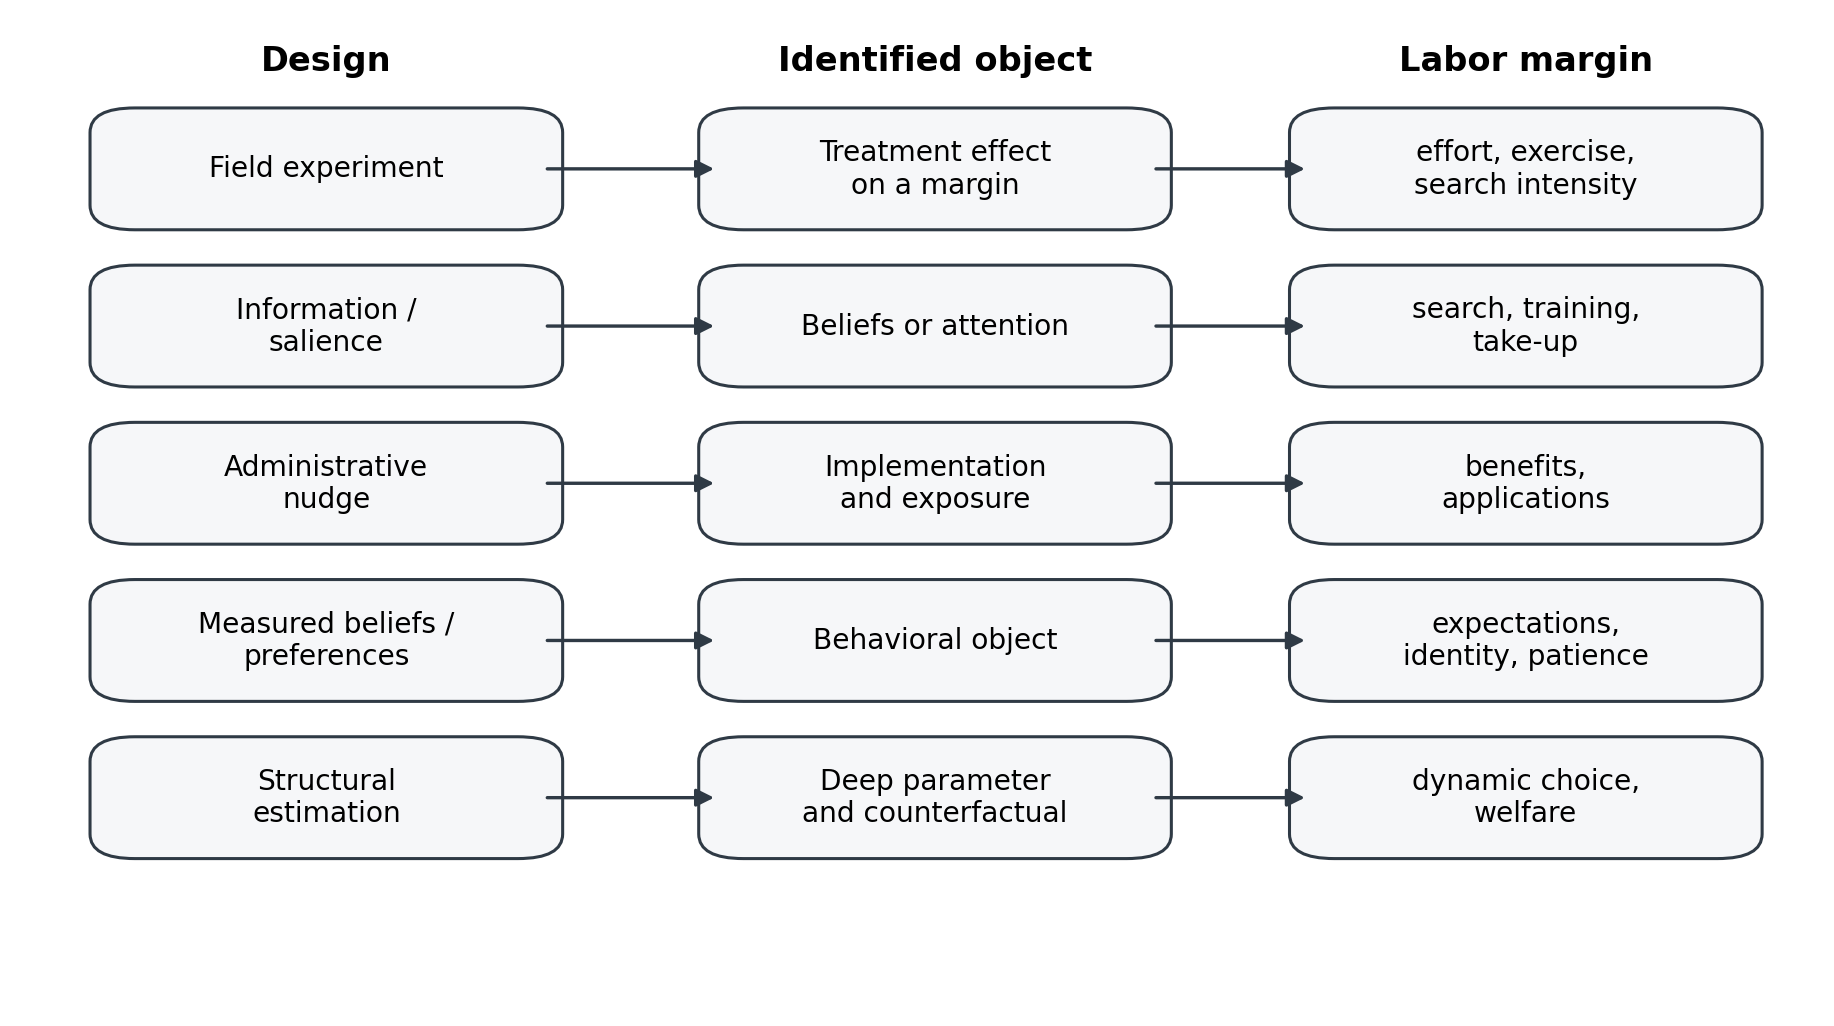
\includegraphics[height=0.78\textheight,keepaspectratio]{01-methods-identification-map.png}
\end{center}
\end{frame}

\begin{frame}{What different designs identify}
\small
\begin{tabular}{p{0.30\linewidth} p{0.32\linewidth} p{0.28\linewidth}}
\toprule
Design & Identified object & Labor use \\
\midrule
Field experiment & Treatment effect on a margin & incentives, effort, search \\
Information intervention & Beliefs or attention & search, training, take-up \\
Administrative nudge & Implementation and exposure & applications, benefits \\
Measured beliefs/preferences & Behavioral heterogeneity & expectations, patience, identity \\
Structural estimation & Parameter and counterfactual & dynamic choice, welfare \\
\bottomrule
\end{tabular}
\end{frame}

\begin{frame}{Welfare and equilibrium cautions}
\[
I_i(a_i^{B}) = V_i(a_i^\dagger) - V_i(a_i^{B})
\]

\begin{itemize}
    \item A behavioral treatment effect is not automatically a welfare gain.
    \item Welfare requires a normative benchmark, internality measure, and account of sophistication.
    \item Firm, market, and policy response can mask, amplify, or reallocate the behavioral wedge.
\end{itemize}
\end{frame}

\begin{frame}{Response before interpretation}
\begin{center}
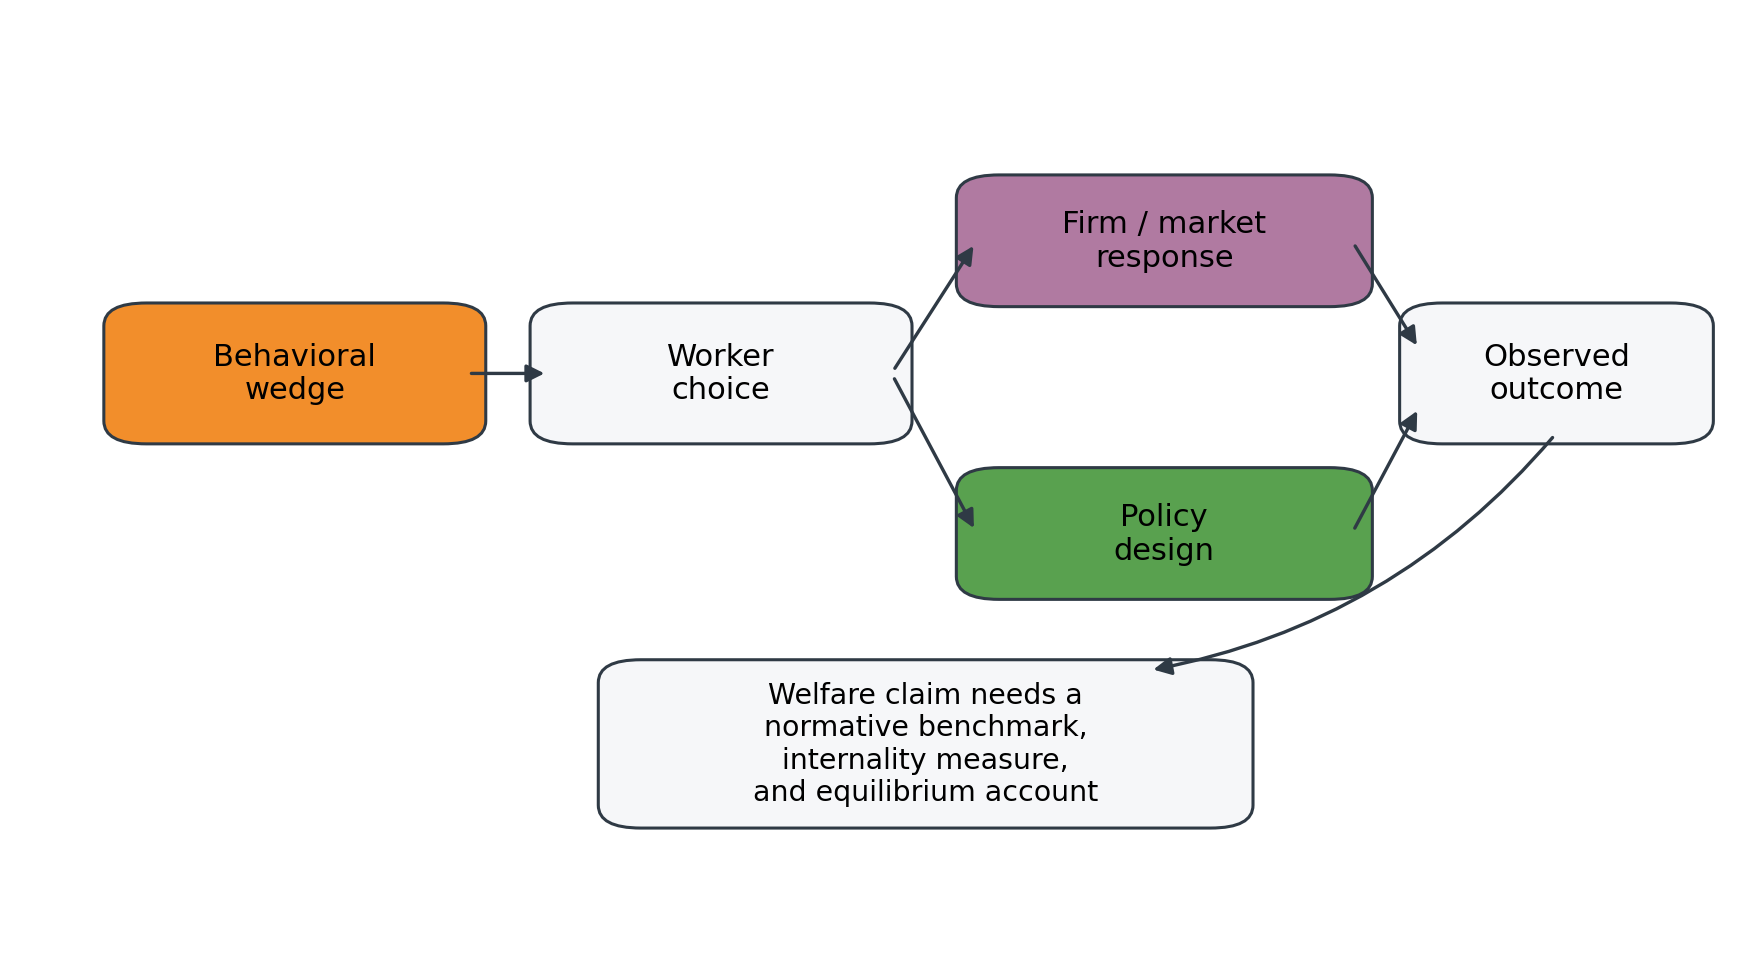
\includegraphics[height=0.76\textheight,keepaspectratio]{01-welfare-equilibrium-caution.png}
\end{center}
\end{frame}

\begin{frame}{Week 1 lab}
\begin{itemize}
    \item Primary anchor: incentives, commitments, and habit formation among workers.
    \item Reproduce: bounded synthetic worker wellness experiment.
    \item Diagnose: separate incentive response, commitment demand, and persistence.
    \item Transfer: apply the same classification logic to a job-search information design.
\end{itemize}
\end{frame}

\begin{frame}{Bridge to Week 2}
\begin{itemize}
    \item Week 1 gives the full map.
    \item Week 2 zooms in on nonstandard preferences.
    \item Central next questions: present bias, reference dependence, reciprocity, social preferences, identity.
    \item The same discipline remains: benchmark, wedge, margin, identification, welfare, response.
\end{itemize}
\end{frame}

\begin{frame}{Takeaways}
\begin{itemize}
    \item Behavioral Labor is labor economics organized around behavioral wedges and design.
    \item The field is strongest when behavioral mechanisms imply distinctive labor predictions.
    \item Methods matter because different designs identify different objects.
    \item Welfare and equilibrium interpretation require more than a positive behavioral effect.
\end{itemize}
\end{frame}

\end{document}
